\documentclass[12pt]{article}
\usepackage{setspace, graphicx, fullpage, amssymb, amsmath, epsfig, natbib, array, multirow, hyperref}
\usepackage{amsfonts, bm} 
\usepackage{dcolumn}
\usepackage{subfigure, float} 
\usepackage[margin=1in]{geometry} 
\usepackage{verbatim}
\usepackage{url}
\usepackage{enumerate}
\newcolumntype{d}[1]{D{.}{.}{#1}} 

\begin{document}
	
\begin{center}
	\Large 01 March 2017
\end{center}

\section{Overview}

At our last meeting, we finally reached full agreement on the use and reasoning of using an \verb|lm| to sort party votes. Further, it was decided that we should produce additional tables and figures of potential interest for developing our analysis based on the additional things we wished to use the Senate to study as well as those which could allow us to more easily compare the House and Senate. Specifically, the following items were selected to see this week:

\begin{itemize}
	\item Create more concise tables showing the signs of coefficients at the end of the vote sorting algorithm
	
	\item Develop plots which show the percent of votes sorted as party calls by Congress\footnote{I also have plots which show the percent of votes which were noncalls by Congress. They are essentially mirror images of the plots I show in this document. If desired, I could also develop gray vote percent plots.}
	
	\item Create coefficient plots for ideological extremism by Congress between a series of groups we want to compare (Democrats/Republicans, Southern/Other Democrats, Gingrich Senators/Other Republicans, Senators approaching election/other Senators, Majority/Minority with Congress 107)
	
	\item The DV/IV and IV/IV plots for House Republicans with the exclusion of the outliers on the right side of the graph
\end{itemize}

\noindent
Each of these is included throughout the rest of this document. Further, I include a regression table for our models of Southern/Other Democrats and Gingrich Senators/Other Repubicans. We should discuss which of these results would be best discussed in the paper and if there are further tests we want to conduct in addition to when we want to begin writing.

\clearpage	

\section{Tables and Figures}
	
\subsection{Sorting Coefficient 2 $ \times $ 2 Tables}

% latex table generated in R 3.3.2 by xtable 1.8-2 package
% Thu Feb 23 17:23:31 2017
\begin{table}[ht]
	\centering
	\caption{Senate Sorting Algorithm Coefficient Signs}
	\begin{tabular}{rrr}
		\hline
		& ($-$) Ideal & (+) Ideal \\ 
		\hline
		($-$) Party & 0.33 & 0.16 \\ 
		(+) Party & 0.23 & 0.28 \\ 
		\hline
	\end{tabular}
\end{table}

% latex table generated in R 3.3.2 by xtable 1.8-2 package
% Thu Feb 23 17:39:42 2017
\begin{table}[ht]
	\centering
	\caption{House Sorting Algorithm Coefficient Signs}
	\begin{tabular}{rrr}
		\hline
		& ($-$) Ideal & (+) Ideal \\ 
		\hline
		(-) Party & 0.38 & 0.15 \\ 
		(+) Party & 0.17 & 0.30 \\ 
		\hline
	\end{tabular}
\end{table}

\clearpage

\subsection{Vote Sorting by Congress}

\begin{figure}[h]
	\centering
	\caption{Senate Party Calls by Congress}
	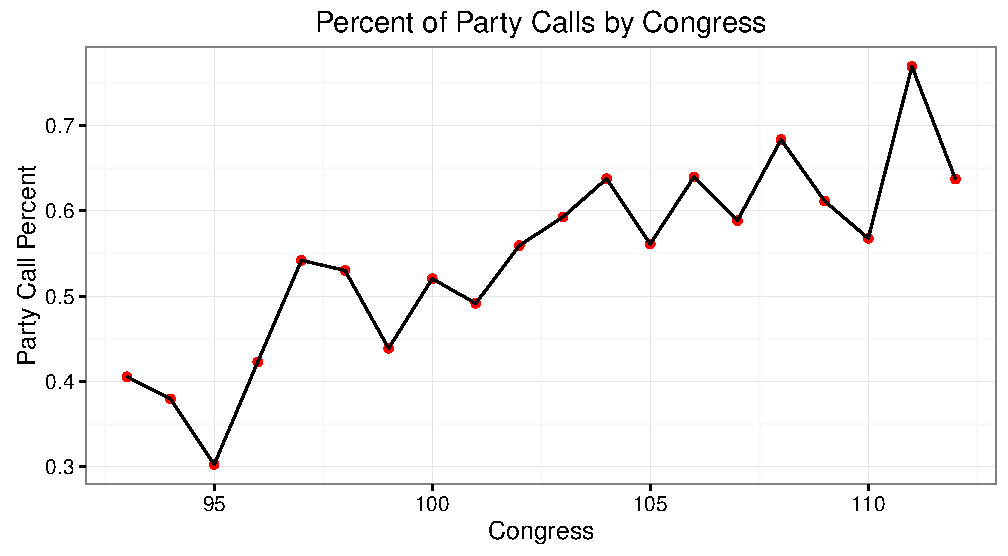
\includegraphics[width = 13cm]{C:/Users/Ethan/Documents/GitHub/partycalls/plots/party_call_percent_plot_senate_lm.pdf}
\end{figure}


\begin{figure}[h]
	\centering
	\caption{House Party Calls by Congress}
	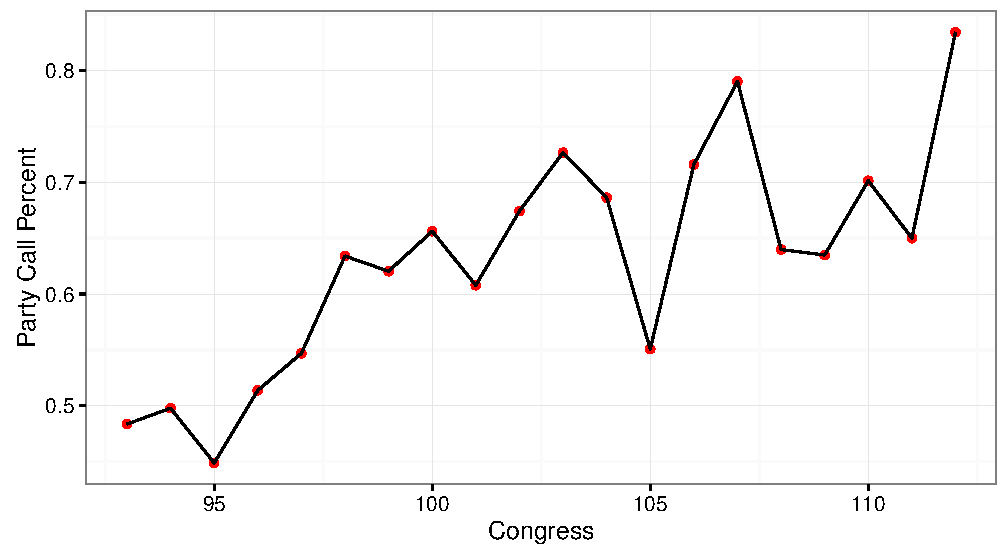
\includegraphics[width = 13cm]{C:/Users/Ethan/Documents/GitHub/partycalls/plots/party_call_percent_plot_house_lm.pdf}
\end{figure}


\clearpage

\subsection{Senate Coefficient Plots}

\begin{figure}[ht]
	\centering
	\caption{Coefficient Plot, Senate Democrats and Republicans}
	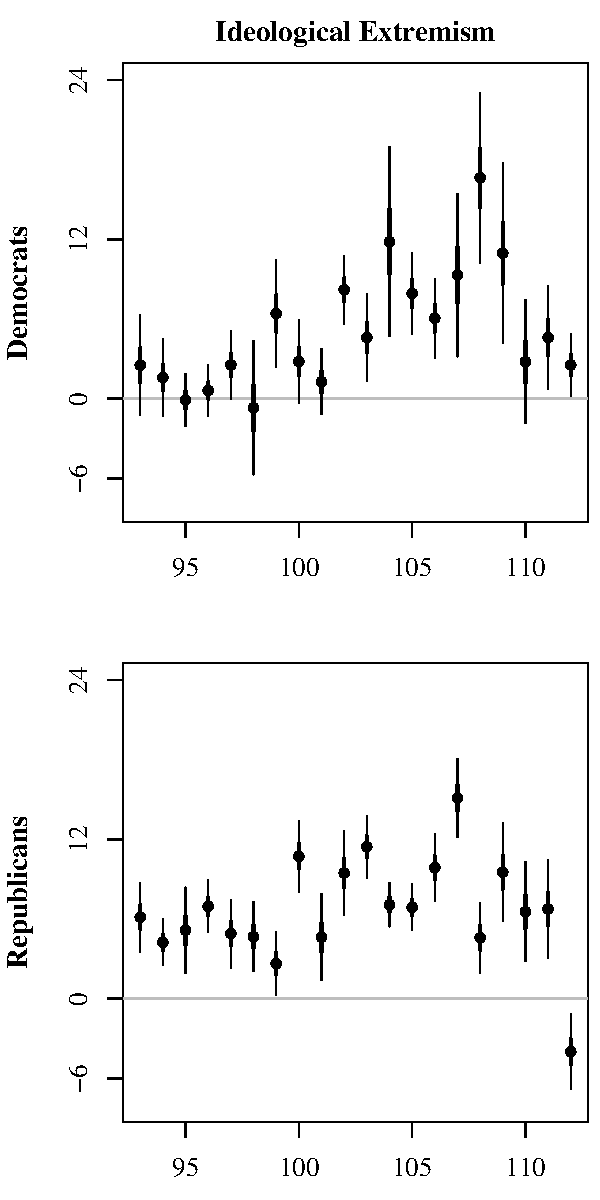
\includegraphics[width = 8cm]{C:/Users/Ethan/Documents/GitHub/partycalls/plots/senate-figure2-party.pdf}
\end{figure}

\begin{figure}[ht]
	\centering
	\caption{Coefficient Plot, Senate Southern and Other Democrats}
	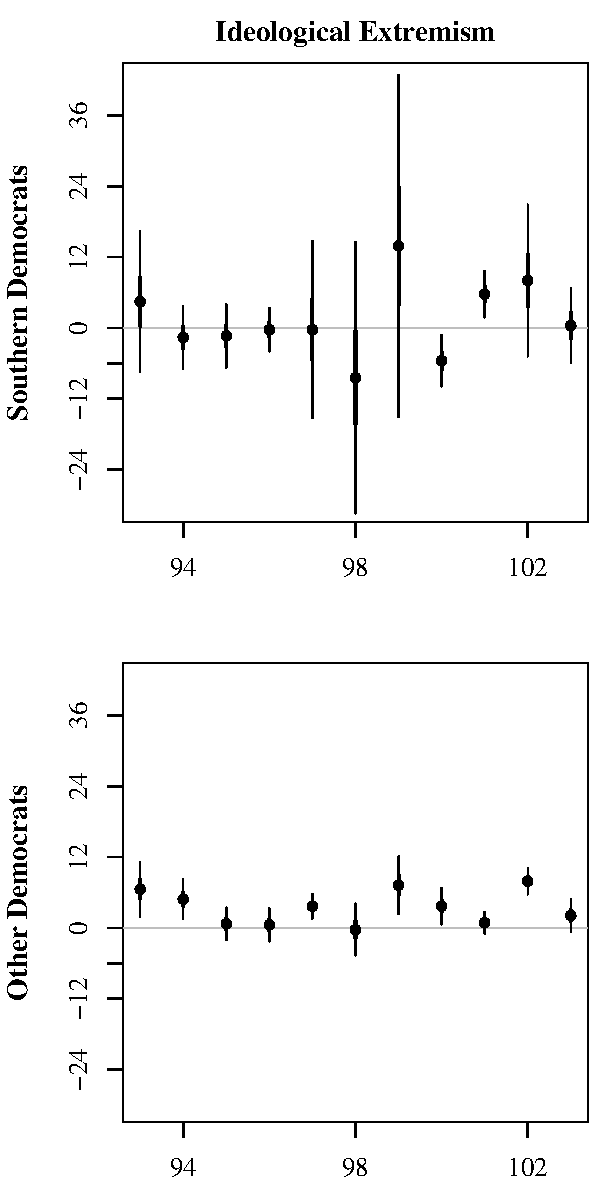
\includegraphics[width = 8cm]{C:/Users/Ethan/Documents/GitHub/partycalls/plots/senate-figure2-southern-other-dems.pdf}
\end{figure}

\begin{figure}[ht]
	\centering
	\caption{Coefficient Plot, Gingrich Senators and Other Republicans}
	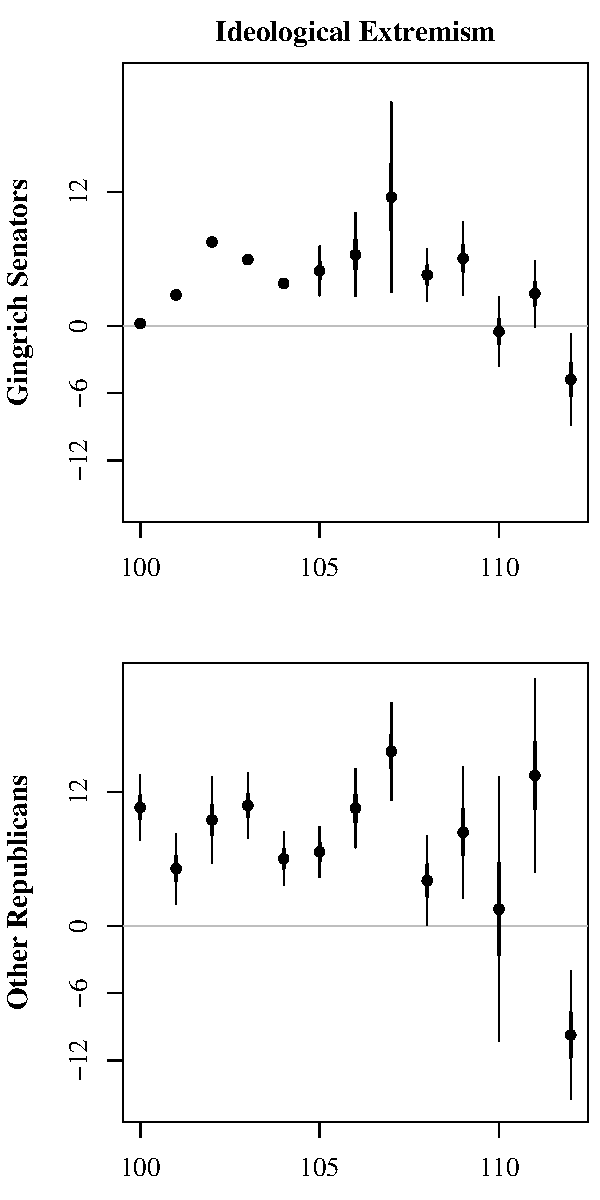
\includegraphics[width = 8cm]{C:/Users/Ethan/Documents/GitHub/partycalls/plots/senate-figure2-gingrich-other-reps.pdf}
\end{figure}

\begin{figure}[ht]
	\centering
	\caption{Coefficient Plot, Senators Up for Reelection and Others}
	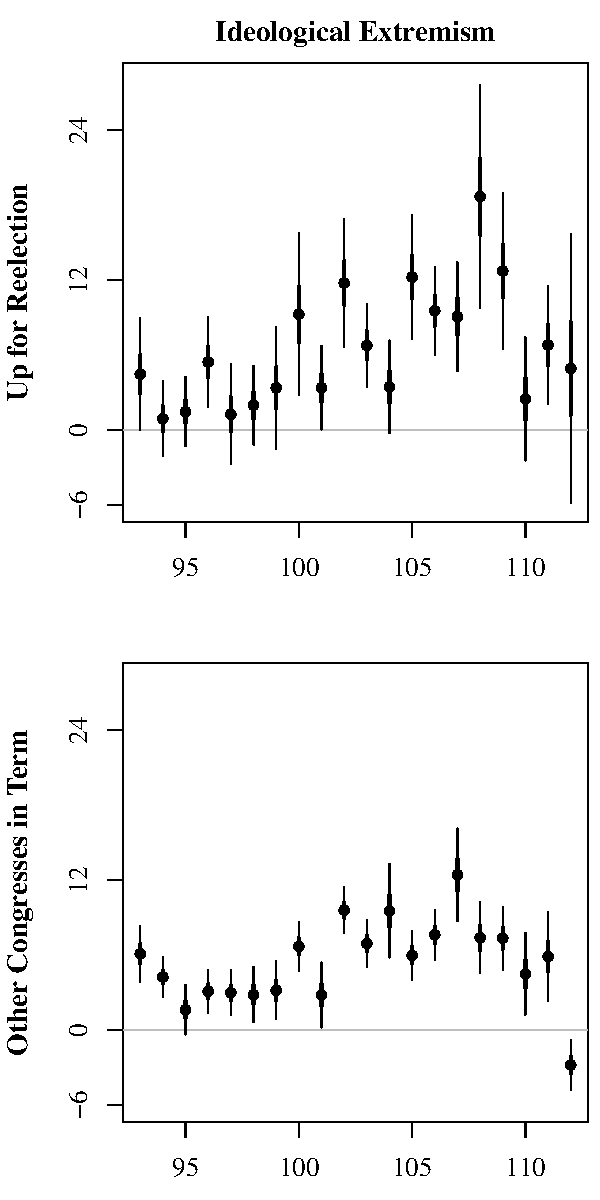
\includegraphics[width = 8cm]{C:/Users/Ethan/Documents/GitHub/partycalls/plots/senate-figure2-reelection.pdf}
\end{figure}

\clearpage

\subsection{House Coefficient Plots}

\begin{figure}[ht]
	\centering
	\caption{Coefficient Plot, House Democrats and Republicans}
	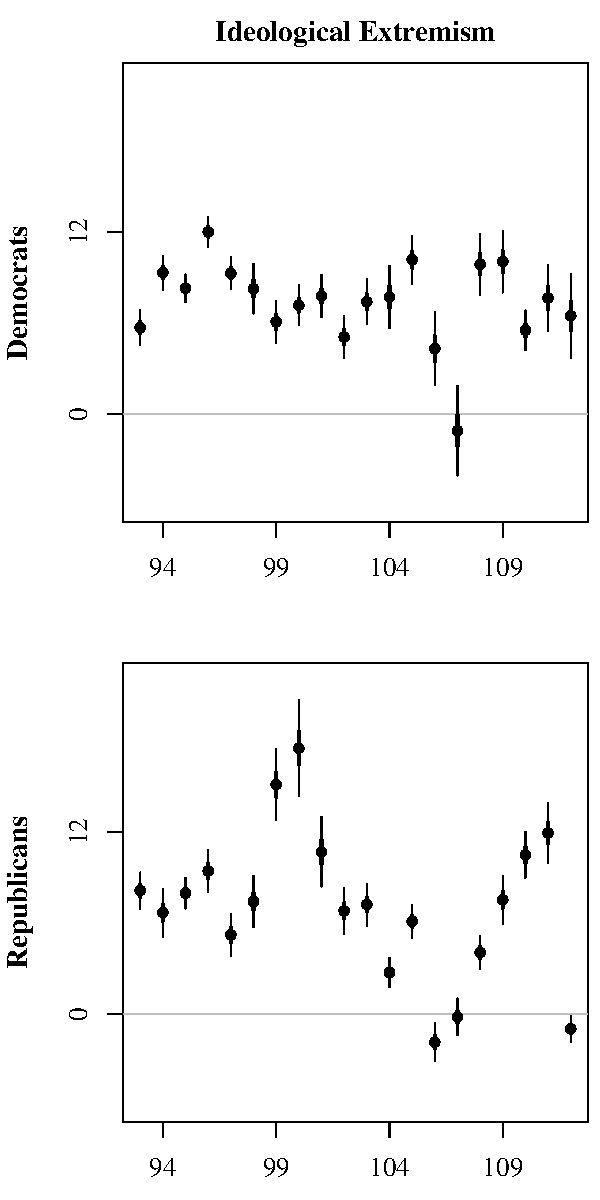
\includegraphics[width = 8cm]{C:/Users/Ethan/Documents/GitHub/partycalls/plots/who-heeds-figure2-replication_party.pdf}
\end{figure}

\begin{figure}[ht]
	\centering
	\caption{Coefficient Plot, House Southern and Other Democrats}
	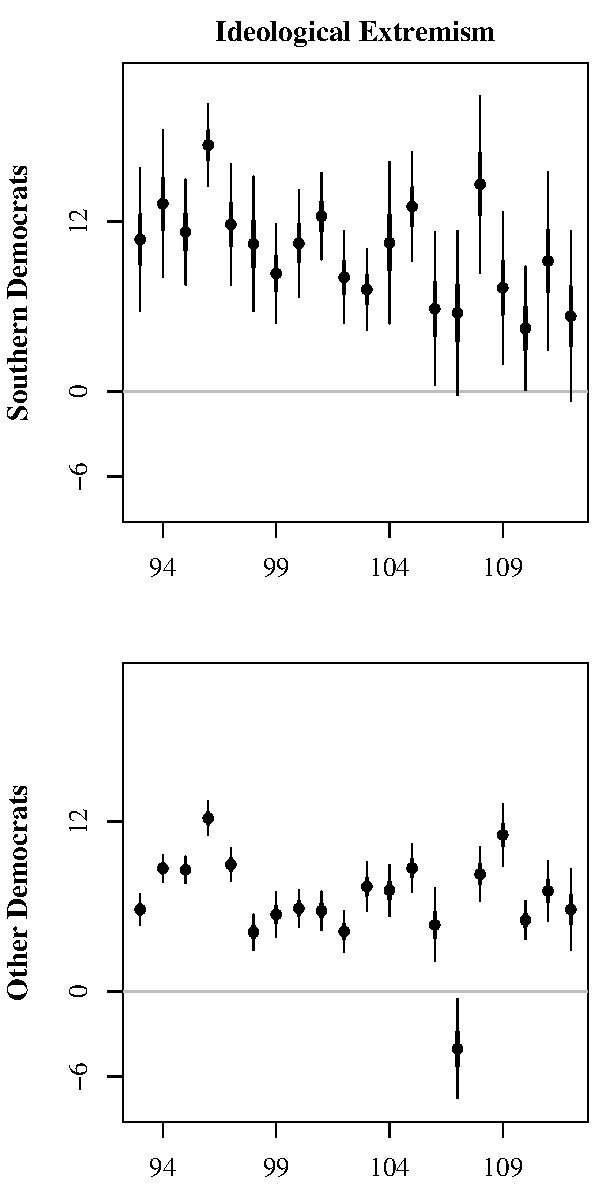
\includegraphics[width = 8cm]{C:/Users/Ethan/Documents/GitHub/partycalls/plots/who-heeds-figure2-replication-south-other-dems.pdf}
\end{figure}

\clearpage

\subsection{Condensed DV/IV and IV/IV Plots, House Republicans}

\begin{figure}[h]
	\centering
	\caption{House Republicans, Ideological Extremism and Party Influenced Vote Rate by Majority Status}
	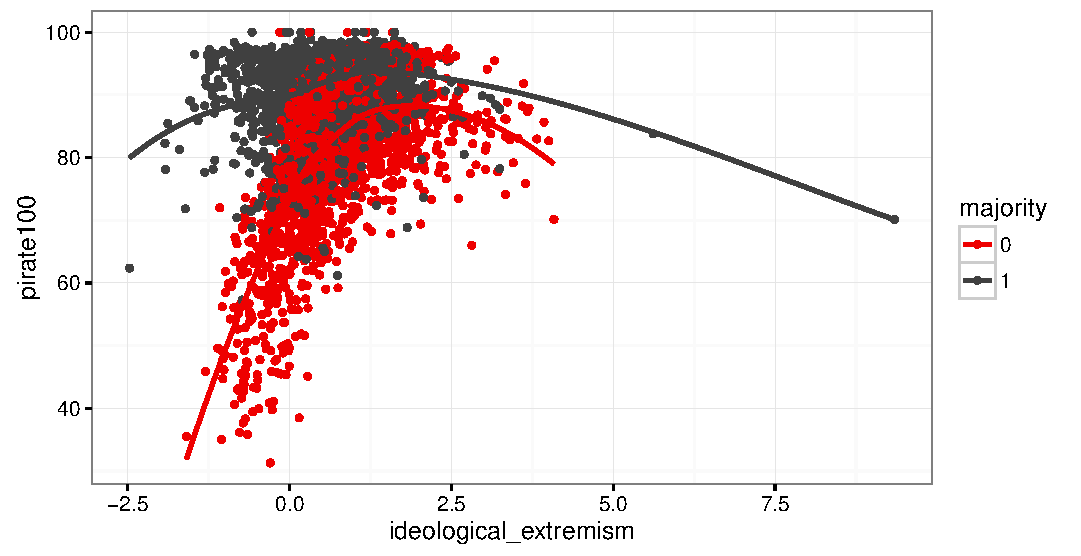
\includegraphics[width = 13cm]{C:/Users/Ethan/Documents/GitHub/partycalls/plots/house_lm_rep_iv-dv_majority.pdf}
\end{figure}


\begin{figure}[h]
	\centering
	\caption{House Republicans, Ideological Extremism and Party Free Vote Rate by Majority Status}
	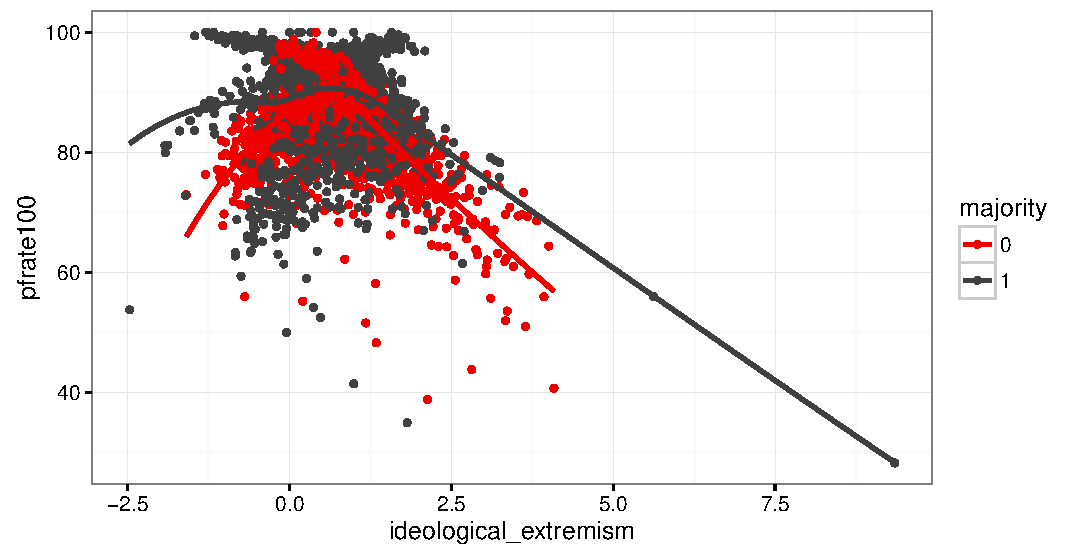
\includegraphics[width = 13cm]{C:/Users/Ethan/Documents/GitHub/partycalls/plots/house_lm_rep_iv-iv_majority.pdf}
\end{figure}

\clearpage

\subsection{Senate Intra-party Comparison Regressions}

\begin{table}[!ht]
	\small
	\begin{center}
		\caption{Senate Intra-Party Comparison Table}
		\begin{tabular}{l c c c c }
			\hline
			 & South. Democrats & Democrats & Gingrich Senators & Republicans \\
			\hline
			Ideological Extremism & $4.657^{***}$  & $2.519^{***}$  & $3.058^{***}$  & $6.570^{***}$  \\
			& $(1.157)$      & $(0.413)$      & $(0.589)$      & $(0.398)$      \\
			South                  &                &                & $0.102$        & $0.811$        \\
			&                &                & $(0.644)$      & $(0.661)$      \\
			Baseline Party Vote Rate              & $0.844^{***}$  & $0.639^{***}$  & $0.293^{***}$  & $0.820^{***}$  \\
			& $(0.066)$      & $(0.035)$      & $(0.046)$      & $(0.034)$      \\
			Pres. Vote Share      & $26.380^{***}$ & $24.044^{***}$ & $-4.157$       & $-5.883$       \\
			& $(5.096)$      & $(2.672)$      & $(4.293)$      & $(3.411)$      \\
			Vote Share            & $-4.027$       & $-4.607$       & $3.928$        & $10.878^{***}$ \\
			& $(3.861)$      & $(2.881)$      & $(3.325)$      & $(3.240)$      \\
			Latino                 &                & $2.734$        & $3.612$        & $3.009$        \\
			&                & $(1.965)$      & $(2.302)$      & $(3.593)$      \\
			Female                 & $0.125$        & $2.404^{**}$   &                & $1.872$        \\
			& $(1.993)$      & $(0.739)$      &                & $(1.115)$      \\
			Up for Reelection    & $-1.645$       & $-0.392$       & $-0.308$       & $-2.041^{***}$ \\
			& $(1.070)$      & $(0.427)$      & $(0.676)$      & $(0.581)$      \\
			Seniority              & $-0.403^{*}$   & $0.048$        & $-0.108$       & $0.249^{**}$   \\
			& $(0.165)$      & $(0.062)$      & $(0.211)$      & $(0.087)$      \\
			Freshman               & $-1.135$       & $-1.310^{*}$   & $0.636$        & $1.937^{*}$    \\
			& $(1.458)$      & $(0.588)$      & $(1.141)$      & $(0.828)$      \\
			Retiree                & $1.867$        & $2.130^{*}$    & $3.060^{*}$    & $2.480^{*}$    \\
			& $(2.249)$      & $(0.946)$      & $(1.468)$      & $(1.044)$      \\
			Best Committee        & $0.460$        & $0.064$        & $-0.225$       & $0.022$        \\
			& $(0.303)$      & $(0.137)$      & $(0.181)$      & $(0.182)$      \\
			Party Leader                 & $5.760^{*}$    & $1.713^{*}$    & $2.004$        & $1.290$        \\
			& $(2.311)$      & $(0.702)$      & $(1.031)$      & $(0.840)$      \\
			Power Committee       & $0.762$        & $-1.179$       & $1.995$        & $-0.760$       \\
			& $(2.110)$      & $(0.797)$      & $(1.029)$      & $(1.061)$      \\
			Committee Chair                  & $3.196^{*}$    & $0.557$        & $1.194$        & $3.889^{***}$  \\
			& $(1.401)$      & $(0.556)$      & $(1.017)$      & $(0.739)$      \\
			African American                   &                & $-0.455$       &                & $-7.396$       \\
			&                & $(2.498)$      &                & $(4.177)$      \\
			(Intercept)            & $-2.038$       & $22.236^{***}$ & $67.517^{***}$ & $7.632$        \\
			& $(7.168)$      & $(3.234)$      & $(5.152)$      & $(4.003)$      \\
			\hline
			R$^2$                  & 0.727          & 0.572          & 0.296          & 0.682          \\
			Adj. R$^2$             & 0.712          & 0.564          & 0.239          & 0.675          \\
			Num. obs.              & 246            & 793            & 187            & 762            \\
			RMSE                   & 7.346          & 5.437          & 3.710          & 7.052          \\
			\hline
			\multicolumn{5}{l}{\scriptsize{$^{***}p<0.001$, $^{**}p<0.01$, $^*p<0.05$}} \\
			\multicolumn{5}{l}{\footnotesize{\textit{Note}: The columns labeled ``Democrats'' and ``Republicans'' do not contain the separately modeled groups}} \\
			\multicolumn{5}{l}{\footnotesize{Southern Democrats and Gingrich Senators.}}
		\end{tabular}
	\end{center}
\end{table}



















\end{document}